\newcommand{\comment}[1]{}

%\documentclass[a4paper,twocolumn,12pt]{article}

%\documentclass[a4wide,12pt]{report}

%\documentclass[a4wide,12pt]{article}
%\documentclass[informasjonssikkerhet]{gucmasterproject}
\documentclass[informationsecurity]{gucmasterproject}

%\usepackage{pslatex} %% Doesn't seem to work - i.e. convert .eps to .pdf
 
\usepackage[utf8]{inputenc}     % For utf8 encoded .tex files
%\usepackage[latin1]{inputenc}
\usepackage[norsk]{babel}     % For chapter headings etc.
%\usepackage[pdftex]{graphicx}           % For inclusion of graphics

%From http://math.uib.no/it/tips/
   %% For grafikk
    \usepackage{ifpdf}
    \ifpdf
      \usepackage[pdftex]{graphicx}
      \usepackage{epstopdf}
    \else
      \usepackage[dvips]{graphicx}
    \fi
    %% Her kan du putte dine vanlige pakker og definisjoner



%\usepackage[dvips]{hyperref}    % For cross references in pdf
\usepackage{hyperref}
\usepackage{mdwlist}
\usepackage{url}
\usepackage{here}

\def\UrlFont{\tt}

\begin{document}

\thesistitle{IMT5391 Service Design - NAV}
\thesisauthor{Engedal, J. Ø., Grimsgaard, C., Pedersen, K.}
\thesisdate{\gucmasterthesisdate}
\useyear{2014}
\makefrontpages % make the frontpages
%\thesistitlepage % make the ordinary titlepage


\comment{
Front page - including
"   HIG technical report front page including logos etc.
"   The text: "MSc project plan"
"   Title of project
"   Name of author and contact details
"   Date
"   Version

email address
"   MAIS students must include "NISlab" as their affiliation.
Date:22.10.2003

Structure of MSc thesis project plan
Gj�vik University College
}




\begin{abstract}
Alderspensjon fra NAV er noe alle nordmenn går i gjennom i løpet av livet sitt. I og med at alderspensjon er så viktig, er målgruppen svært stor, og det er utfordrende for tjenester som skal være tilpasset flere forskjellige brukergrupper. I historien om en far, en sønn og et esel av den greske fabelforfatteren Æsop \cite{aesop}, fortelles det om hvordan ingen av de forbipasserende var fornøyd med hvem som satt på eselet. Moralen fra fabelen kan trekkes inn i prinsipper for universell utforming, og lærer oss at dersom man prøver å gjøre alle fornøyd, gjør man ingen fornøyd. NAV har gjennom flere år hatt et dårlig rykte på seg, så vi interesserte oss for å finne ut om NAVs tjeneste løste utfordringene som følger med en så stor brukerbase.

For å evaluere NAV sin alderspensjonstjeneste har vi brukt metoder som stakeholderanalyse, kundereisediagram, personas, scenarioer og intervju. I tillegg har vi analysert IT-systemene som er i bruk og reflektert rundt NAVs løsning. Vi kom frem til at dagens løsning fungerer godt og trenger ingen restrukturering av service designen, men presentasjonen av alderspensjon på NAV sitt nettsted har potensiale til å bli forbedret. Fra intervjuer og bruk av personas og scenario oppdaget vi en manglende oppsummering av alderspensjon. Det var størst behov hos de unge brukerne som ikke ønsket å lese om alle de kompliserte reglene om alderspensjon, men heller ønsket en rask introduksjon til hva alderspensjon er, hvordan man opptjener alderpensjon og annen nødvendig informasjon om alderspensjon. Vi har produsert et løsningsforslag som vil kunne hjelpe NAV med å nå frem til unge brukere ved å rette opp i disse forbedringspunktene.

\end{abstract}


\tableofcontents


 \chapter{Introduksjon}
I denne oppgaven har vi valgt å se nærmere på emnet pensjon og da mer spesifikt på hvordan informasjonen til tjenestene rundt alderspensjon fungerer. Disse tjenestene er alle tilgjengelige via nettsidene til NAV. Vi har valgt å fokusere på brukeropplevelser knyttet til nettstedet til NAV og utbetaling av pensjon gjennom bruk av fiktive brukere og intervjuer med ekte brukere. 


\chapter{Dagens løsning hos NAV}
\section{Refleksjon rundt NAV}
Vi ønsker å ta for oss hvordan informasjon om alderspensjon blir presentert på NAV sine nettsider. Vår analyse vil ha hovedfokus på nettsiden til NAV og ta for seg hvordan informasjonen blir presentert. Analysen vår baserer seg på metodene presentert nedenfor og spørsmål rundt hvordan man opptjener alderspensjon, hvordan man får pengene utbetalt og generell presentasjon av innhold.

NAV sine nettsider består hovedsaklig av informasjon og tjenester knyttet til de fire hovedemnene arbeid, familie, pensjon og helse. Vi har valgt å ta for oss pensjon, og da spesifikt alderspensjon. I denne rapporten vil vi se på allerede eksisterende service design ved å gjennomføre analyser og vurdere potensielle tiltak som vil forbedre dagens løsninger. NAV.no tilbyr i dag muligheter via sin løsning “Din pensjon” for å beregne pensjon, se pensjonsopptjening, bruke pensjonskalkulator og søke om alderspensjon.

I 2013 ble det registrert 1,8 millioner besøk hver måned på internett, 8,2 mill. samtaler årlig til kontaktsentre, flere millioner besøk årlig ved personlig oppmøte og det blir sendt 22 mill. dokumenter årlig til NAV via post. NAV har i følge samme undersøkelse 456 kontorer i forskjellige kommuner og bydeler. I følge samme undersøkelse mottok 760 000 personer alderspensjon. 57 000 av dem var under 67 år, mens 65 prosent kombinerte jobb og pensjon. Av disse, jobbet 78 prosent heltid \cite{faktaogtall}.

Pensjon som emne er veldig bredt da det finnes flere typer pensjon avhengig av hvilken situasjon man er i. Det finnes uførepensjon, krigspensjon, ytelser ved dødsfall, tjenestepensjon og omsorgsopptjening. Vi har valgt å se nærmere på alderspensjon fordi dette er en ordning alle må innom i løpet av livet sitt. Det er den eldre brukergruppen som mottar alderspensjon og denne brukergruppen har ofte vanskeligheter med syn og motorikk. Eldre er med andre ord en interessant og noe krevende brukergruppe å ha med og gjøre på grunn av de mange kravene som de har. Vi kan nesten anse denne brukergruppen for det som kalles “edge-case”. Det betyr at hvis den eldre brukergruppen klarer å bruke tjenesten tilnærmet optimalt, vil andre og mindre krevende brukergrupper heller ikke ha problemer med tjenesten. Samtidig er pensjonssidene på NAV.no ikke bare beregnet for eldre, men alle aldersgrupper. Fordi reglene rundt pensjon er så mange og kompliserte, er ikke unge nødvendigvis så interessert i å lese om pensjon. Ved å se på alderspensjon vil vi kunne se om behovet for den eldre brukergruppen tilfredsstiller, og om den yngre brukergruppen får informasjon slik de ønsker.



\section{Analyse av stakeholders}
Stakeholdere er de som blir direkte eller indirekte påvirket av organisasjonens handlinger, mål og politikk \cite{stakeholder}.
\begin{itemize}
\item Alle fremtidige eller nåværende mottakere av pensjon
\item De som har tilknytning til pensjonsmottakere
\item NAV som organisasjon
\item NAV-ansatte
\item Stat
\item Kommune
\item Politiske partier
\end{itemize}

Antallet alderspensjonister forventes å overstige 1 million i 2020, i følge NAVs egne tall \cite{antallpassert}. Pensjonstjenesten vil med andre ord havne under større press, og det er i allmenn interesse at tilbudet oppleves som tilfredsstillende, både av mottakere så vel som deres familie og venner. NAV har opplevd en del negativ medieoppmerksomhet i senere tid, og ansatte har blitt utsatt for trusler og sjikane; det er derfor betydelig interesse for at organisasjonen oppnår et forbedret rykte, som følge av vel utformede tilbud.

NAV er et statlig tilbud, så det er betydelig politisk interesse med i bildet, så vel som spørsmålet om trygghet forbundet med offentlige tjenester. Det er en viss frykt og negativitet forbundet med alderdom, så langsiktig sett er det i allmennhetens interesse å ha en trygg og positiv alderdom å se frem til.



\section{Personas}
\subsection{Thomas Larsen}
\textbf{Navn:} Thomas Larsen \\
\textbf{Alder:} 24 \\
\textbf{Yrke:} Elektriker \\
\textbf{Sivilstand:} Ugift \\
\textbf{Utdanning:} Yrkesfaglig med fagbrev \\
\textbf{Forhold til NAV mtp alderspensjon:} Lever i sin egen verden med lite kjennskap til hvordan alderspensjon fungerer og sin rolle i det. Stoler på arbeidsgiver. \\
\textbf{Teknisk kompetanse:} Gjennomsnittlige IT-kunnskaper. Har en iPad som brukes mest for underholdning. \\
\textbf{Beskrivelse:} Thomas Larsen jobber i Elektriske A/S som holder til i Stavanger. Han leier en leilighet der han bor sammen med hunden sin. På fritiden liker han å spille fotball og går jevnlig på Viking-kamper sammen med kompiser. Han bruker iPhone 5 og iPad til å holde kontakt med venner via sosiale medier, samt til underholdning via enkle spill på iPad. Har en gammel Acer laptop som brukes veldig lite, der han bruker Google Chrome som sin valgte nettleser. Har ingen tidligere erfaringer med NAV. Det eneste han vet om alderspensjon er at arbeidsgiver betaler inn en hvis prosentandel av utbetalt lønning. Tenker svært lite på alderspensjon siden han er såpass ung og ikke har trengt å tatt stilling til dette enda. \\
\textbf{Mål:} Ønsker seg mer informasjon om hvordan man tjener opp til alderspensjon. \\


\subsection{Gudrun Bekkehavn}
\textbf{Navn:} Gudrun Bekkehavn \\
\textbf{Alder:} 44 \\
\textbf{Yrke:} Lærer på barneskole \\
\textbf{Sivilstand:} Gift med Arne Bekkehavn \\
\textbf{Utdanning:} Lærer utdanning på høgskolenivå + et par fag som etterutdanning \\
\textbf{Forhold til NAV mtp alderspensjon:} Har god kontroll over sin alderspensjonsplan. Har hatt “veiledningsmøter” med NAV og fått god informasjon innenfor dette. \\
\textbf{Teknisk kompetanse:} Det at hun er ansvarlig for IT-opplæringen ved skolen, gjør at hun har god kontroll på tekniske løsninger. \\
\textbf{Beskrivelse:} Gudrun og Arne holder til i Fredrikstad i et stort hus. De har to barn, Jarle på 23 og Silje på 20. Gudrun er mye opptatt med sin lærerrolle og setter pris på fritiden hun har. Derfor liker hun å være effektiv i dagligdagse gjøremål. Hun er ofte innom NAV på Din Side for å sjekke diverse informasjon og holde tritt på sin egen alderspensjonsplan. \\
\textbf{Mål:} Ønsker å sjekke status på sin opptjente alderspensjon.


\subsection{Pål Wolfgang}
\textbf{Navn:} Pål Wolfgang \\
\textbf{Alder:} 63 \\
\textbf{Yrke:} Kundebehandler ved DNB (20\%) \\
\textbf{Sivilstand:} Gift med Mia Wolfgang \\
\textbf{Utdanning:} Økonomi og ledelse ved UiO \\
\textbf{Forhold til NAV mtp alderspensjon:} Er i ferd med å alderspensjonere seg og har dialog med NAV vedørende utbetaling og overgangen til aktiv alderspensjonisttilværelse. \\
\textbf{Beskrivelse:} Pål er en godt likt kundebehandler som er i ferd med å alderspensjonere seg. Han har nettopp flyttet inn i ny leilighet, sentralt i Oslo sentrum sammen med sin hustru. Han har gode IT-kunnskaper som han har lært seg via diverse kurs relevante til sin jobb som kundebehandler. Akkurat nå skal han bli alderspensjonist og gleder seg til å ta tidlig alderspensjon. \\
\textbf{Mål:} Ønsker å gå av med alderspensjon og få sin første utbetaling.


\section{Scenarioer}
\subsection{Thomas Larsen}
Thomas ønsker mer informasjon om hvordan alderspensjon beregnes og lurer på om det er noen regler rundt alderspensjon han har behov for å vite i sin alder.

Thomas skal besøke bestemoren sin i Arendal og sitter på toget fra Stavanger. Mens han hører på musikk på iPhonen, tenker han på hvor mye han vanligvis reiser i løpet av et år og undrer seg over hvor mye han kommer til å kunne reise som pensjonist. Siden han ikke har noe bedre å gjøre, drar han opp iPaden fra sekken og åpner nettleseren Safari. Han navigerer seg til www.nav.no i håp om å finne enkel og kortfattet informasjon om alderspensjon. Øverst på siden finner han hovedmenyen og trykker på “Pensjon”. Siden han blir presentert med forvirrer han og han er usikker på hvor han skal sette blikket. Han oppfatter midtdelen av siden som en blanding av en footer og en blogg, og snur blikket mot høyresiden av nettsiden. Der finner han lenker til tjenester som en forenklet pensjonskalkulator og en mulighet å se sin pensjonsopptjening. Han ønsker ikke å legge inn noe data og leter heller videre etter relevant informasjon. I menyen til venstre finner han menyelementet “alderspensjon” og trykker det. Igjen synes Thomas at nettsiden er merkelig konstruert, men har lært fra forrige side at kanskje det han leter etter finner han i venstremenyen. Der ser og trykker han på et undermenyelement som heter “Om alderspensjon”. Dette tar han til en side spekket med tekst, men det var forsåvidt det han lette etter. Det første paragrafet oppsummerer hva alderspensjon er. Han skumleser videre gjennom det neste paragrafet, men begynner heller å se på underoverskriftene på nettsiden for å se om det er noe relevant. Han ble ikke helt tilfredsstilt. Han ser i venstremenyen igjen og finner noe som heter “Opptjening” og trykker seg videre. Han skumleser gjennom den første punktlisten og ser at hans alderspensjonsopptjening følger de nye reglene. Han ser etter underoverskriften som har med nye regler å gjøre. Han finner det og begynner å lese. Det andre listepunktet var akkurat det han lette etter! Her står det kort og godt hvordan man opptjener alderspensjon. Thomas føler ikke for å lese mer om alderspensjon. Han skrur av iPaden, legger den i sekken og går tilbake til å høre på musikk.

\subsection{Gudrun Bekkehavn}
Gudrun er årlig innom “Ditt NAV” på www.nav.no for å sjekke diverse informasjon og holde tritt på sin egen pensjonsplan, og nå er tiden kommet for å gjøre nettopp det.

Gudrun er på jobb og har en ledig time. Hun setter seg foran arbeidsdatamaskinen sin og navigerer seg til www.nav.no. Hun er godt kjent på siden og vet hvor hun skal. Hun navigerer seg videre til “Pensjon” gjennom hovedmenyen og til høyre på siden finner hun tjenesten om å se sin pensjonsopptjening. Hun klikker lenken og logger seg inn via fødselsnummer, passord og engangskode på SMS. Når hun er inne på “Ditt NAV” finner og klikker hun på undermenyelementet til venstre som heter “Din pensjonsoppdatering”. Der blir hun presentert med en liste over hennes pensjonsoppdatering år for år. Hun bekrefter at all informasjon er som antatt og dobbeltsjekker tallene fra siste år. Hun er fornøyd og lukker nettleseren.

\subsection{Pål Wolfgang}
Pål er i ferd med å pensjonere seg og har dialog med NAV vedrørende utbetaling og overgangen til aktiv pensjonisttilværelse. Han har over lang tid visst pensjonsreglene som gjelder han, men fordi han nylig bestemte seg for å ta ut pensjon tidligere enn han tenkte i utgangspunktet, ønsker han å vite hvor mye han vil få utbetalt ved å pensjonere seg tidlig.

Han sitter i stua en kveld med iPaden i fanget og navigerer seg til www.nav.no i Safari. Nettstedet er kjent siden han har vært der mange ganger før. Han finner hovedmenyen og trykker på “Pensjon”. Han ønsker å se hvor mye han vil få utbetalt gjennom tidlig pensjon, så han klikker på “Se din pensjonsopptjening” til høyre på siden. Nettstedet presenterer en innloggingsbeskjed som krever MinID. Dette hadde han glemt. Han husker ikke hvor han har lagt innloggingsinformasjonen og bestemmer seg for å gjøre det senere. På forrige side la han allikevel merke til en annen lenke som het “Forenklet pensjonskalkulator”. Han tenker at den vil kunne gi han en viss idé. Han navigerer seg tilbake ett hakk og klikker “Forenklet pensjonskalkulator” i samme boks som tidligere. Han fyller ut data etter beste evne og klikker “Beregn pensjon”. Han får en feilmelding om at han hadde glemt å fylle inn data i et felt og retter fort opp feilen. Han klikker “Beregn pensjon” igjen. Siden presenterer en tabell og en fargefylt graf som viser hans inntekt som pensjonist. Han er fornøyd med resultatet, men kommer allikevel til å prøve igjen når han finner innloggingsinformasjonen til MinID så han får et mer nøyaktig estimat.

\section{Intervju}
Vi har tatt kontakt med pensjonister og foretatt korte og ustrukturerte intervjuer for å kartlegge hvordan de opplever NAVs pensjonstjeneste. Samtlige pensjonister hadde møtt opp på NAV sine kontorer og søkt om pensjon via skriftlige skjemaer. Ingen hadde benyttet seg av NAV sine nettsider da det var mange år siden de gikk ut med pensjon og NAV hadde ikke samme tilbud på det tidspunktet. Hver måned får pensjonistene tilsendt et brev fra NAV som inneholder kvittering på pensjonen for den måneden. Samtlige pensjonister vi intervjuet var fornøyd med tjenesten og hadde ikke hatt noen problemer.

I tillegg har vi intervjuet representanter fra den yngre brukergruppen. Disse intervjuene viste at svært få visste hva alderspensjon var og hvordan man opptjente det. De som ble intervjuet informerte om at dette var noe arbeidsgiver tok seg av, noe avtalefestet pensjon (AFP) gjør. Ingen av de spurte visste at det var NAV som faktisk betalte ut pensjon når man er ferdig i arbeidslivet og skal pensjonere seg. Vi informerte om at NAV på sin nettside informerer om alderspensjon og gav dem en oppgave som gikk ut på å finne ut mer om hva pensjon er. Formålet med oppgaven var å finne ut hvordan disse brukerne ville gå frem for å skaffe seg nok informasjon til å føle seg trygge på hva pensjon er.
Alle brukerne navigerte seg frem til hovedsiden til pensjon uten problemer. Hovedsiden bød derimot på enkelte problemer for noen av brukerne. De forstod ikke hvilken informasjon som var viktig i forhold til definisjon av hva alderspensjon er. De oppfattet informasjonen som ble presentert som uryddig og ustrukturert. De mer nettvante brukerne oppdaget at lokalmenyen til venstre hadde en undermeny der det stod nettopp alderspensjon. Ved å trykke på lenken, ble brukerne ledet til en informasjonside som forklarte om alderspensjon.

De fleste middelaldrende har fått informasjon om pensjon gjennom arbeidsgiver, og er i god rute med å spare opp pensjon. Disse ønsker å følge opp sin spareplan og følge med på sin fremtidige utbetalingsplan. De eldste, som er i overgangen mellom jobb og pensjonisttilværelse \textbf{[ }.

\subsubsection{Beskrivelse av innhold - Forside pensjon}
Headeren inneholder en link til en animasjonsfilm som prøver å forklare hvordan man tjener opp pensjon. Global meny og andre verktøy som snarveier og søkefelt er plassert øverst på siden. Selve innholdet som gjelder pensjon er presentert ved en lokal meny til venstre, 3 forskjellige linker til tjenester her representert ved en kombinasjon av bilder og tekst, en tabell om aktuelle tema, en tabell om ting som er nyttige å vite, enda en tabell som viser til forskjellige tjenester til høyre, og aktuelle nyheter på bunnen.
Vi ser tydelig at informasjonen er plassert rundt i flere blokker, noe som gjør siden uoversiktlig og uryddig. Vi ser også at er komplisert å se hva som blir ønskes fremhevet av informasjon. NAV ser ut til å ta utgangspunkt i at alt er like relevant og viktig, og at poenget er å få frem mest mulig informasjon på én side.



\section{Kundereise}

\begin{figure}[h!]
	\centering
	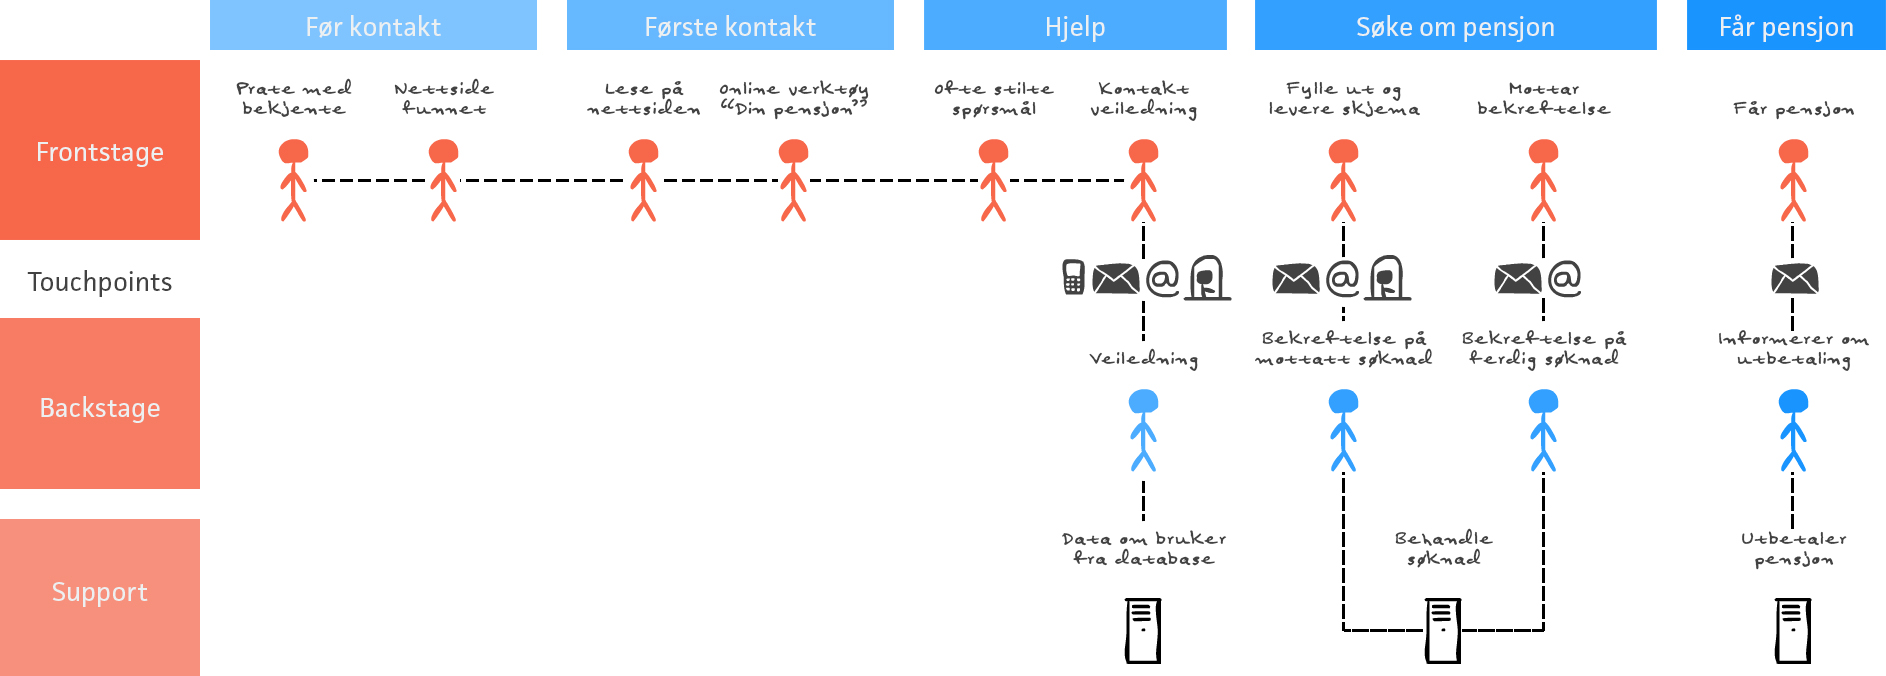
\includegraphics[width=59em, angle=270]{kundereise}
	\caption{Kundereisen visualisert.}
	\label{fig:kundereise}
\end{figure}

Her er en skriftlig beskrivelse av kundereisen.(1) betyr det som kalles frontstage. Dette er det brukeren gjør, ser og opplever. (2) står for backstage, som er det NAV gjør som brukeren ikke er spesielt oppmerksom på. Mellom (1) og (2) er det som kalles touchpoints; der brukeren møter NAV. Her nevner vi også på hvilken måte brukeren er i kontakt med NAV. (3) står for de hjelpelige prosessene, som f.eks. datasystemer, databaser osv.

\subsubsection{Før kontakt}
\begin{itemize}
\item (1) Prate med bekjente
\item (1) Nettside funnet
\end{itemize}

\subsubsection{Første kontakt}
\begin{itemize}
\item (1) Lese på nettsiden
\item (1) Online verktøy “Din alderspensjon”
\end{itemize}

\subsubsection{Hjelp}
\begin{itemize}
\item (1) Ofte stilte spørsmål
\item (1) Kontakter veiledning
	\begin{itemize}
	\item Telefon
	\item Fysisk
	\item Epost
	\item Post
	\end{itemize}
\item (2) Veileder
\item (3) Data om bruker fra database
\end{itemize}

\subsubsection{Søk om alderspensjon}
\begin{itemize}
\item (1) Fylle ut og levere skjema
	\begin{itemize}
	\item Post
	\item Fysisk
	\end{itemize}
\item (2) Bekreftelse på mottatt søknad
\item (3) Behandle søknad
\item (2) Bekreftelse på ferdig søknad
	\begin{itemize}
	\item Epost
	\item Post
	\end{itemize}
\end{itemize}

\subsubsection{Får utbetalt alderspensjon}
\begin{itemize}
\item (3) Utbetaler alderspensjon
\item (2) Informerer om utbetaling
	\begin{itemize}
	\item Post
	\end{itemize}
\item (1) Får alderspensjon
\end{itemize}



\section{Metoder}
\subsection{Generelt om metodene}
For å få et innblikk i hvordan tilbudet til NAV oppleves, benyttet vi oss av et knippe brukersentrerte metoder for å få et innblikk i hvordan andre enn oss selv opplever tjenesten. NAV står overfor betydelige organisasjonelle utfordringer, og tallene er der ute; vi ønsker å ta for oss de menneskelige og ikke-målbare aktørene og prosessene i organisasjonen.

\subsection{Personas}
Pensjon er en såpass generell og allmenngjeldende tjeneste, så det kan bli noe vanskelig å se for seg spesifikke enkelttilfeller og problemene man kan støte på. Ved å lage et sett personas tilegnet vi oss en bredere forståelse av hvordan ofte beskrevne frustrasjoner ved NAV kan komme til uttrykk.

Personaene våre fungerte godt som et virkemiddel for oss internt, slik at vi fikk visualisert problemene vi har avdekket i oppgaven vår, samtidig som de kan bidra til å kommunisere problemområder lettere enn tung fagterminologi.

\subsection{Stakeholder-analyse}
Ved å gjennomføre en slik analyse fikk vi dannet oss et overblikk av NAV utenom fagspesifikke ting. Vi opplevde det som interessant å ta større samfunnsrelaterte spørsmål i betraktning, og følte at det å ha et helhetlig og vidt perspektiv i prosessen hjalp å belyse viktige momenter, som ikke nødvendigvis ville ha blitt avdekket dersom vi hadde fokusert kun på NAV eller pensjon.

\subsection{Intervju}
Metoden er en sentral del i brukersentrerte prosesser - det oppfordres stadig til å snakke med brukerne. Intervjuene våre avslørte at selve pensjonstjenesten egentlig ser ut til å være ganske godt utformet.

Vi fikk dessuten kartlagt problematikken forbundet med å tilegne seg informasjon relatert til pensjon, og unges mangel på kunnskap mtp hvordan pensjonsordningen fungerer i praksis.

Ved å gjennomføre intervjuer fikk vi innsyn i hvor problemområdene ligger, slik at vi kunne utarbeide løsninger. Intervjuene bød også på informasjon som var interessant, og kan komme oss til gode ved senere anledninger.

\subsection{Kundereise}
For å kartlegge og visualisere hvilke elementer som inngår i selve pensjonssøkingsprosessen lagde vi en kundereiseoversikt. Tanken var å se hvorvidt det finnes enkelte steg som er til hindring for brukere mtp måloppnåelse, men vi fant ingen problemer.



\chapter{Refleksjon}
Service Design handler om å designe brukervennlige og konkurransedyktige løsninger basert på brukernes behov. I Service Design-prosessen vil man kartlegge brukernes ferd i det aktuelle systemet eller tjenesten. Prosessen kan variere avhengig av hva slags kompleksitet og størrelse det er på organisasjonen og tjenesten som tilbys. Ettersom NAV er en stor offentlig organisasjon, er det betydelige utfordringer når det gjelder brukskvaliteten til IT-systemet som brukes.

Ofte når man designer og utvikler nye IKT systemer, blir oppgaven for kompleks og utfordrende. Dette skyldes i stor grad mangel på forståelse av IT og kompleksiteten i store prosjekter. Nylig ble et delprosjekt av NAVs moderniseringsprosjekt av IT systemene deres stoppet etter å brukt 700 millioner kroner \cite{stansetprosjekt}. Målet for dette prosjektet er å få til en felles IT-platform som erstatter den nåværende tunggrodde IT-platformen som i dag består av 300 ulike datasystemer. I dette tilfellet ble utviklerne for ambisiøse, som daglig leder Joakim Lystad sier: “Men i ettertid ser vi at vi var for ambisiøse, og at vi ikke så kompleksiteten i å samordne den nye plattformen med de eksisterende løsningene og ordningene”.

Utfordringer knyttet til store IKT-løsninger finner vi også i helsesektoren. Oslo-sykehusene hadde et prosjekt som gikk ut på å lage et felles grensesnitt mot de forskjellige IKT-systemene som ble brukt. Dette prosjektet måtte avbrytes etter forsinkelser, og kostnadene ble anslått til å være over 160 millioner. Det ble av enkelte antydet at prosjektet hadde en urealistisk tidsramme.

Disse to eksemplene viser at store prosjekter ikke alltid blir gjennomført og må avbrytes, mye på grunn av forsinkelser eller uforutsette problemer ved implementering. Disse prosjektene kaster bort verdifulle ressurser uten å tilføre nye løsninger. Utfordringene er mange og slike prosjekter lider av at de rett og slett er for store og komplekse.

\begin{quote}
''Den største jobben ligger i prosessen med å ta teknologien i bruk og tilpasse den til organisasjonen, og med å tilpasse organisasjonen og arbeidsfordelingen og rutinene til det teknologien krever og muliggjør'' \cite{aanestad}.
\end{quote}

Sett fra et sosioteknisk perspektiv, er overføring fra ett medium til et annet ikke nødvendigvis bedre. IKT-prosjekter blir ofte sett på som løsningen på et aktuelt problem, men fører ofte til enda større problemer enn situasjonen bydde på i utgangspunktet. En måte å se dette på, er digitalisering av systemer som ofte fører til økt grad av sosioteknisk kompleksitet. Hvis det for eksempel ligger en bunke papirer i en bestemt hylle på et sykehus, så vil enkelte arbeidsprosesser settes i gang. Hvis man fjerner dette fysiske signalet, må man altså finne en måte å gjengi symbolikken i den digitale verden. Løsningen kan være å ha bestemte digitale postkasser til spesifikke formål, slik at brukerne av systemet enkelt kan fange opp meldinger. Hvis dette ikke gjøres, kan slike symboler blir glemt og systemet kan oppleve forsinkelser. Manglende overføring av symbolikk som dette kan være med på å gjøre arbeidsdagen vanskeligere for brukerne av systemet. NAV har tilsvarende utfordringer med tanke på at det er forskjellige systemer som skal kunne kommunisere med hverandre, både lokalt og nasjonalt.

Hva kan man gjøre med det?
Det er viktig å forstå at det er flere aktører i spill når det gjelder såpass store og komplekse IKT-systemer. God planlegging og realistiske målsettinger må være i fokus. Testing må skje i lukkede og isolerte miljøer, for å forsikre at systemet er klart for implementering.
Derfor må man være ekstra grundig i forhåndsarbeidet, der man ser på mer realistiske endringer, samt erkjenner, minimerer og håndterer risiko. Eventuelle feil og problemer kan spres og forårsake store forsinkelser, noe som er en svært aktuell problemstilling når det gjelder NAV.




\chapter{Analyse av IT-systemer}
\section{Grunnleggende analyse}
En enkel analyse av hvilke IT-systemer NAV bruker lar seg vanskelig gjennomføre, ettersom de benytter seg av 300 ulike IT-systemer fordelt på 12 hovedkategorier \cite{sokelys}. Sett bort fra spesifikke tilfeller, kan man resonnere seg frem til at kompleksiteten i seg selv muligens er det mest kritiske problemet. Dersom dette ikke adresseres, vil selv store forbedringer i ett enkelt system være ubetydelige. Dette er ikke nødvendigvis et problem som kommer fra manglende IT-kompetanse, men kanskje en konsekvens av selve organisasjonen og dens allestedsværende og sterkt regulerte natur.

Hva brukeropplevelsen av NAVs IT-systemer angår, foregår det meste i bakgrunnen. Kommunikasjon foregår gjennom telefon, e-post, eller personlig oppmøte - med andre ord, de vanlige kommunikasjonskanalene man forventer i møte med de fleste tjenester. Våre undersøkelser tilsier at pensjonsutbetalinger er forholdsvis uproblematiske i praksis, og krever minimal dialog med etaten. Relevante informasjonsteknologiske komponenter for pensjon på NAV er som følger:

\subsubsection{Touchpoints}
\begin{itemize}
\item Hjemmeside
\item Telefon
\item E-post
\item Lokalt kontor
\item Saksbehandler
\end{itemize}

\subsubsection{Frontstage (den synlige delen)}
\begin{itemize}
\item Hjemmeside
\item Lokalt kontor med medarbeidere
\item Informasjon/nyheter om pensjon
\end{itemize}

\subsubsection{Backstage (den usynlige delen)}
\begin{itemize}
\item Saksbehandling
\item Organisering /koordinasjon/samhandling
\end{itemize}

\subsubsection{Support}
\begin{itemize}
\item Infrastruktur
\item Databaser
	\begin{itemize}
	\item All informasjon vedrørende alle tjenester
	\item Profilhåndtering (login, personlige innstillinger, søknader)
	\item Søknader og andre dokumenter
	\item Kommunikasjon (e-post-systemer, telefoner, nyheter på hjemmeside)
	\end{itemize}
\end{itemize}


\section{CSCW-matrise}
\subsection{Samme sted, samme tid}
Dette er systemene som inngår i forbindelse med personlig oppmøte hos NAV. Selve backend-en kan antas å være den samme som ved andre sanntidsinteraksjoner over f.eks. telefon, som for eksempel registrering eller endring av personopplysninger. Alle slags databasesamhandlinger kan på en måte innordnes under alle de fire forskjellige punktene, ettersom de utgjør en sentral del av et hvert CSCW-scenarie.

Det vil sannsynligvis være de NAV-ansatte som blir nødt til å forholde seg til IT-systemer ved personlige oppmøter, ettersom noe av formålet ved å fysisk oppsøke NAV kan tenkes å være beleiligheten forbundet ved å slippe å måtte forholde seg til uforståelige IT-systemer eller forvirrende fagterminologi.

\subsection{Samme tid, forskjellig sted}
NAV tilbyr en rekke forskjellige muligheter for stedsuavhengig sanntidskommunikasjon. Dersom personlig oppmøte ikke er mulig eller er upraktisk, vil sannsynligvis telefonsamtaler være alderspensjonisters foretrukne løsning. Stedsuavhengigheten er en fordel for alderspensjonisten, men telefonmediet medfører visse vansker for den NAV-ansatte:
\begin{itemize}
\item Lydkvaliteten over telefon er dårlig.
\item alderspensjonister snakker ofte sykt utydelig.
\item Henvisninger til nettadresser eller skjemaer blir vanskelig, ettersom disse har kompliserte navnformater, og NAV-systemet er ganske komplekst for mannen i gata (og NAV-ansatte) å navigere.
\end{itemize}

NAVs chat-funksjonalitet er foreløpig en prøveordning for de som ønsker informasjon angående foreldrepenger, men det kan godt tenkes at NAV vil kunne tilby sanntidsekspertise innen deres andre tilbudsområder også. Merk våre ord - alderspensjonschat vil være en realitet innen 2020.

\subsection{Forskjellig tid, samme sted}
Dette kan muligens være en slags digital informasjonstavle i resepsjonen, eller annen informasjon som endres dynamisk, og skal aksesseres av de NAV-ansatte. Hvis man tolker begrepet bokstavelig, kan muligens en serie av personlige oppmøter være på forskjellig tid og samme sted.

\subsection{Forskjellig tid, forskjellig sted}
Steds- og tidsuavhengig elektronisk kommunikasjon vil hovedsaklig innebære e-post-kommunikasjon, eller NAV-spesifikke meldingssystemer. Sistnevnte har ikke vi tilgang til, og ingen av de vi spurte har uttrykt behov for å kommunisere med NAV på denne måten. E-postkorrespondansen vi selv opplevde var litt lite responsiv, men det kan tenkes at interne løsninger foretrekkes, og at de som faktisk er inne i systemet prioriteres.





\chapter{Løsningsforslag}
Ved å bruke metodene nevnt i del 1 har vi oppdaget en del mangler ved dagens eksisterende løsning. Hovedsaklig gjelder dette informasjonstrømmen til brukerne vedrørende temaet pensjon, via innholdet som er presentert på nettsiden og hvordan den blir presentert. Denne delen av rapporten vil bli brukt til å presentere forslag til forbedringer.

For å oppsummere analysen i del èn, avdekket vi at NAV sine nettsider er generelt veldig rotete, i form av veldig mange hyperlinker på hver side. Spesielt forsiden lider av dette, der linker i global meny og lokal meny fører til samme sted. Eksempelvis er det minst 4 forskjellige lenker som fører til Min Sides innloggingside. Analysen viser også at informasjonen som presenteres er ganske uvilkårlig. Generell informasjon, nyheter, spesielle vilkår, med flere er eksempler på informasjon spredt rundt på sidene.




\begin{figure}[h!]
	\centering
	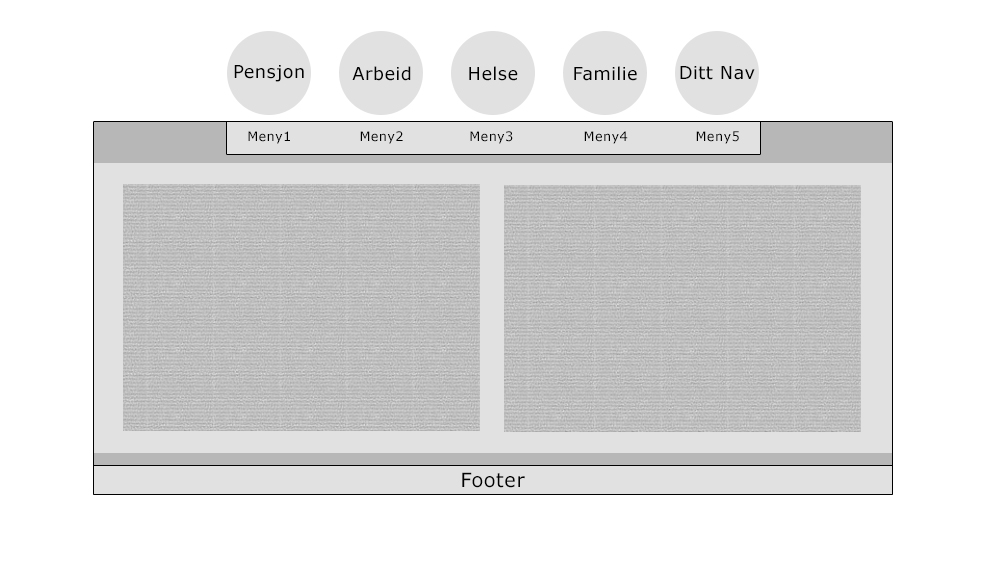
\includegraphics[width=40em]{Skisse_1}
	\caption{Foreslått redesign av menystruktur. Den venstrestilte menyen er gjort om til en toppmeny.}
	\label{fig:skisse1}
\end{figure}




Bakgrunn for figur \ref{fig:skisse1}:
Vi mener at NAV sine nettsider trenger en redesign, da den nåværende nettsiden blir oppfattet som utdatert og uryddig. Hyperlenker dominerer og det er vanskelig å navigere seg til riktig side med relevant informasjon.  Vi foreslår å bruke flere visuelle virkemidler for å hjelpe brukerne, og da spesielt eldre, i og navigere seg frem til riktig side med relevant innhold. Informasjonen som presenteres bør således også restruktureres.

 Vi har igjennom våre analyser kommet frem til følgende punkter vi mener kan være med på å både forenkle budskapet NAV ønsker og formidle, i tillegg til en styrket brukeropplevelse.

\begin{itemize}
\item Et nytt moderne responsivt rammeverk vil forbedre informasjonsflyten og fokus på viktig innhold.
\item Økt fokus på global meny fører til at det blir enklere å navigere.
\item To hovedvinduer vil presentere relevant informasjon (dette kan endres avhengig av hva som presenteres).
\item Footer har quicklinks som: Hjelp, kontakt oss, veiledning (kan også inkluderes som en egen knapp i global meny som f. eks “Hjelp”).
\item Vi ønsker å minimere bruken av hyperlinker ved og plassere dem under dropdown meny fra lokal meny.
\item Vi foreslår å bruke flere symboler eller bilder for å kjapt og enkelt kunne informere brukerne av nettsiden hva informasjonen representerer.
\end{itemize}
Ovenfor liste nevner kun områder som er innenfor de visuelle rammene. Da det gjelder ren organisering av innhold, vil vi komme med følgende råd til utviklerne av NAV.
\begin{itemize}
\item Kutte ned på bruken av kontekstuelle lenker.
\item Sære regler og andre spesielle tilfeller kan gå i egen kategori i undermenyen.
\item Fakta og statistikk kan dyttes ut i en egen “nyttig å vite”.
\end{itemize}

\begin{figure}[h!]
	\centering
	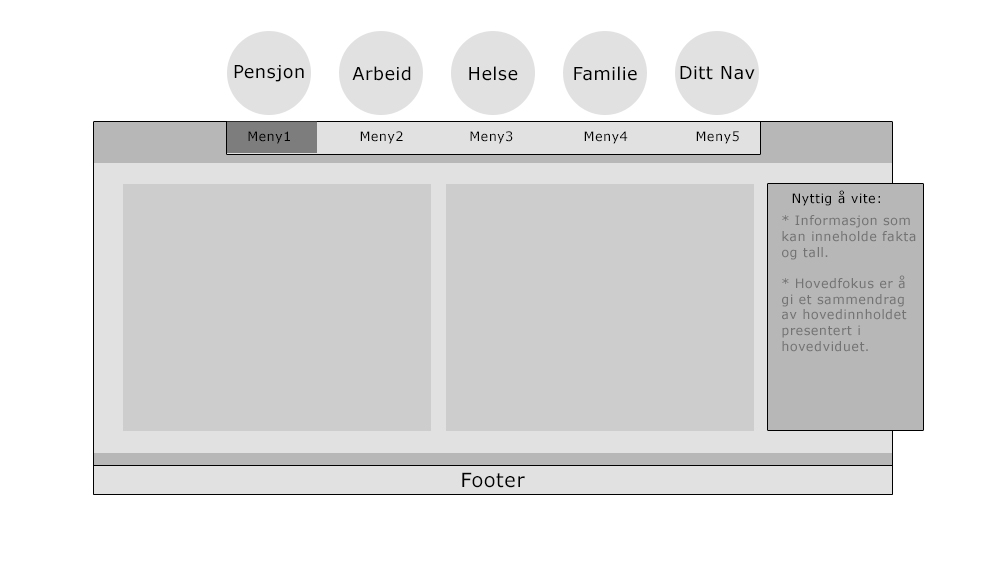
\includegraphics[width=40em]{Skisse_2}
	\caption{Informasjonsboks lagt til på høyresiden for enkel oppsummering av innhold.}
	\label{fig:skisse2}
\end{figure}

Bakgrunn for figur \ref{fig:skisse2}:
\begin{itemize}
\item Informasjonen vil i all hovedsak presenteres så enkelt som mulig
\begin{itemize}
\item “Nyttig å vite” skal gi et overblikk over teksten som presenteres i hovedvinduene
\item Kan bytte på hva som vises, f. eks fakta og tall, historie, ting å være oppmerksom på
\end{itemize}
\end{itemize}

\chapter{Konklusjon}
Selv om NAV er en kompleks entitet, vil nok pensjonssøkere bare oppleve systeminteraksjoner med en brøkdel av de aktuelle systemene. Vi har forsøkt å komme i kontakt med NAV for å undersøke hva slags spesifikke systemer de benytter seg av, men vi har ikke fått svar. Vi har derfor sett oss nødt til å hente inn informasjon om NAV sine systemer fra andre hold.

Når det kommer til selve pensjonstjenesten, høres det egentlig ut som det meste fungerer fint. Prosessen oppleves som lettforståelig og ukomplisert, og ingen av besteforeldrene våre har problemer med NAV når det kommer til pensjon.

Det kan muligens stilles spørsmål ved nødvendigheten av å ha alt av informasjon tilgjengelig på nett. Risikoen for brukerfeil reduseres ved å ha en NAV-ansatt til stede, i motsetning til en setting hvor man selv er nødt til å finne ut av hva som menes ved informasjonen på et stort og komplisert nettsted. Ved personlig oppmøte vil man kun bli presentert relevant informasjon, mens man ved et nettstedsbesøk på eget initiativ blir nødt til å navigere gjennom NAV-jungelen. Informasjonsteknologi er ikke en erstatning for situasjonsforståelsen og kommunikasjonen som en kvalifisert og medfølende person vil kunne vise.



\begin{thebibliography}{9}

\bibitem{aesop}
	Wikipedia.
	\emph{Æsops fabler.}
	http://no.wikipedia.org/wiki/\%C3\%86sops\_fabler
	(sett 11.06.2014)

\bibitem{tallogfakta}
	NAV
	\emph{Nav i fakta og tall 2013.}
	https://www.nav.no/Om+NAV/\_attachment/\\341361?\_ts=146194a3c50
	(sett 11.06.2014)

\bibitem{stakeholder}
	Service Design Tools
	\emph{Stakeholders.}
	http://www.servicedesigntools.org/taxonomy/term/17
	(sett 11.06.2014)

\bibitem{antallpassert}
	NAV
	\emph{Antall alderspensjonister har passert 800 000.}\\
	https://www.nav.no/Om+NAV/Tall+og+analyse/Pensjon/Alderspensjon/Alderspensjon/\\Antall+alderspensjonister+har+passert+800+000.369406.cms
	(sett 11.06.2014)

\bibitem{stansetprosjekt}
	Dagens Næringsliv
	\emph{Nav stanset IT-prosjekt etter å ha brukt 700 mill.}
	http://www.dn.no/nyheter/politikkSamfunn/2014/01/23/nav-stanset-itprosjekt-etter-a-ha-brukt-700-mill
	(sett 11.06.2014)

\bibitem{aanestad}
	Aanestad, M.
	\emph{IKT: Et utfordrende redskap, kapittel 9.}

\bibitem{sokelys}
	Søkelys på samfunnet.
	\emph{Nav under lupen}
	http://sokelys.origo.no/-/bulletin/show/821802\_nav-under-lupen?ref=checkpoint
	(sett 11.06.2014)

\end{thebibliography}






\end{document}